\newpage
\section{Spezifikation}
Basierend auf dem entwickelten Konzept und den definierten Anforderungen wird die detaillierte Spezifikation des Systems ausgearbeitet. Diese umfasst die Architektur des gesamten Systems, welche die Aufteilung in einzelne Komponenten und deren Interaktion untereinander beschreibt. Ebenso wurden die Schnittstellen zwischen den Komponenten definiert. Weiterhin wird erläutert, wie das System mit seiner Umgebung interagiert. Die technische Spezifikation umfasst die verwendete Hardware sowie die eingesetzten Protokolle und Standards, die für Umsetzung der einzelnen Komponenten benötigt werden. 

Zur besseren Veranschaulichung des Gesamtsystems, Beziehungen zwischen den Komponenten und der Abläufe wurden, wo sinnvoll, Diagramme erstellt. Diese visualisieren bestimmte Zusammenhänge. Bei der Erstellung dieser Diagramme wurde das SA/RT-Entwurfskonzept als Orientierungshilfe genutzt. Aufgrund der des hohen Umfangs bzw. der Komplexität des Projekts wurden die strengen Vorgaben des SA/RT-Konzepts jedoch flexibel gehandhabt und nicht strikt befolgt.

\subsection{Architektur}
Die Architektur des Projekts bietet eine Gesamtdarstellung des Systems und zeigt, wie die verschiedenen Komponenten miteinander interagieren. Das System gliedert sich in drei Hauptbereiche: Audioverarbeitung, Benutzeroberfläche (User Interface) und das neuronale Netz.

\begin{itemize}
    \item Systemarchitektur: Gesamtdarstellung des Systems, wie Komponenten zusammenarbeiten
    \item Unterteilung in 3 Komponenten (Audio, User Interface, NN)
    \item Hier SA/RT Kontextdiagramm (evtl. ein Gesamt-Diagramm und pro Komponente ein weiteres)
    \item Hier SA/RT Modell für Zustandsautomat? und ggf. weitere Modelle
    
    \begin{figure}[H]
    	\centering
    	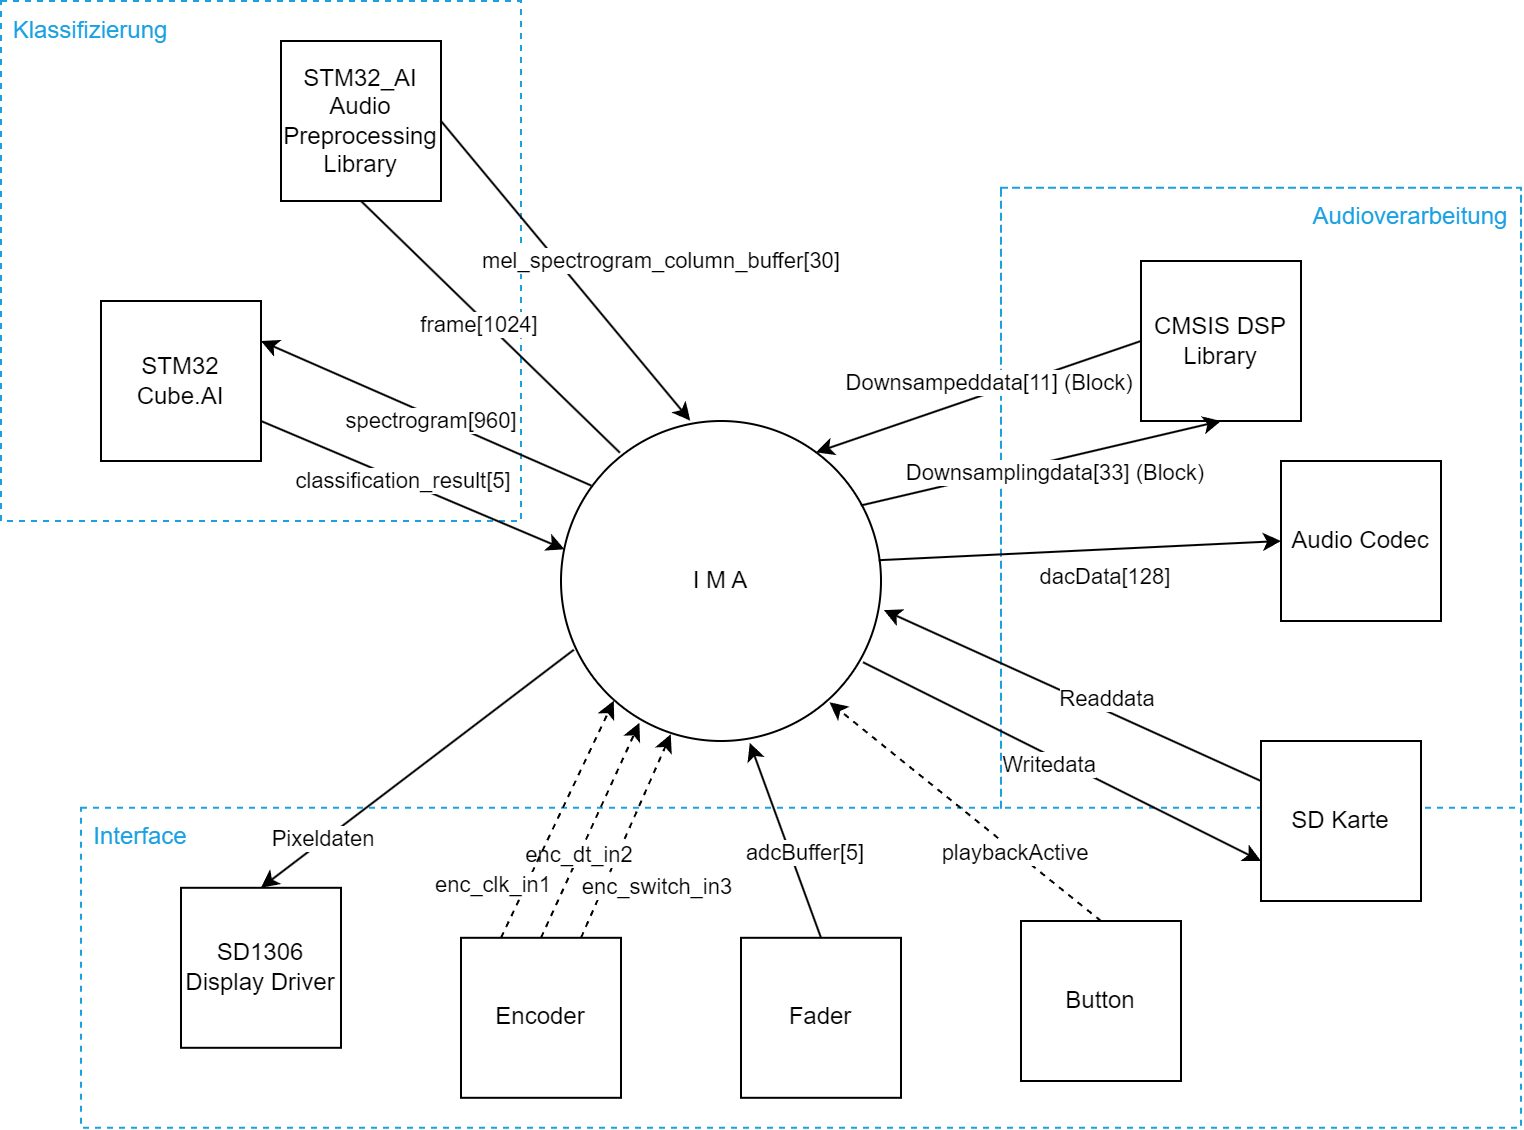
\includegraphics[width=0.8\textwidth]{images/04_spezifikation/kontextdiagramm_gesamt.drawio.png}
    	\caption{Kontextdiagramm des Gesamtsystems}
    	\label{fig:context_diagram_gesamt}
    \end{figure}
    
    %TODO: ausformulieren
    
    %TODO: Kontextdiagramme pro Untersystem
   
    
    \begin{figure}[H]
    	\centering
    	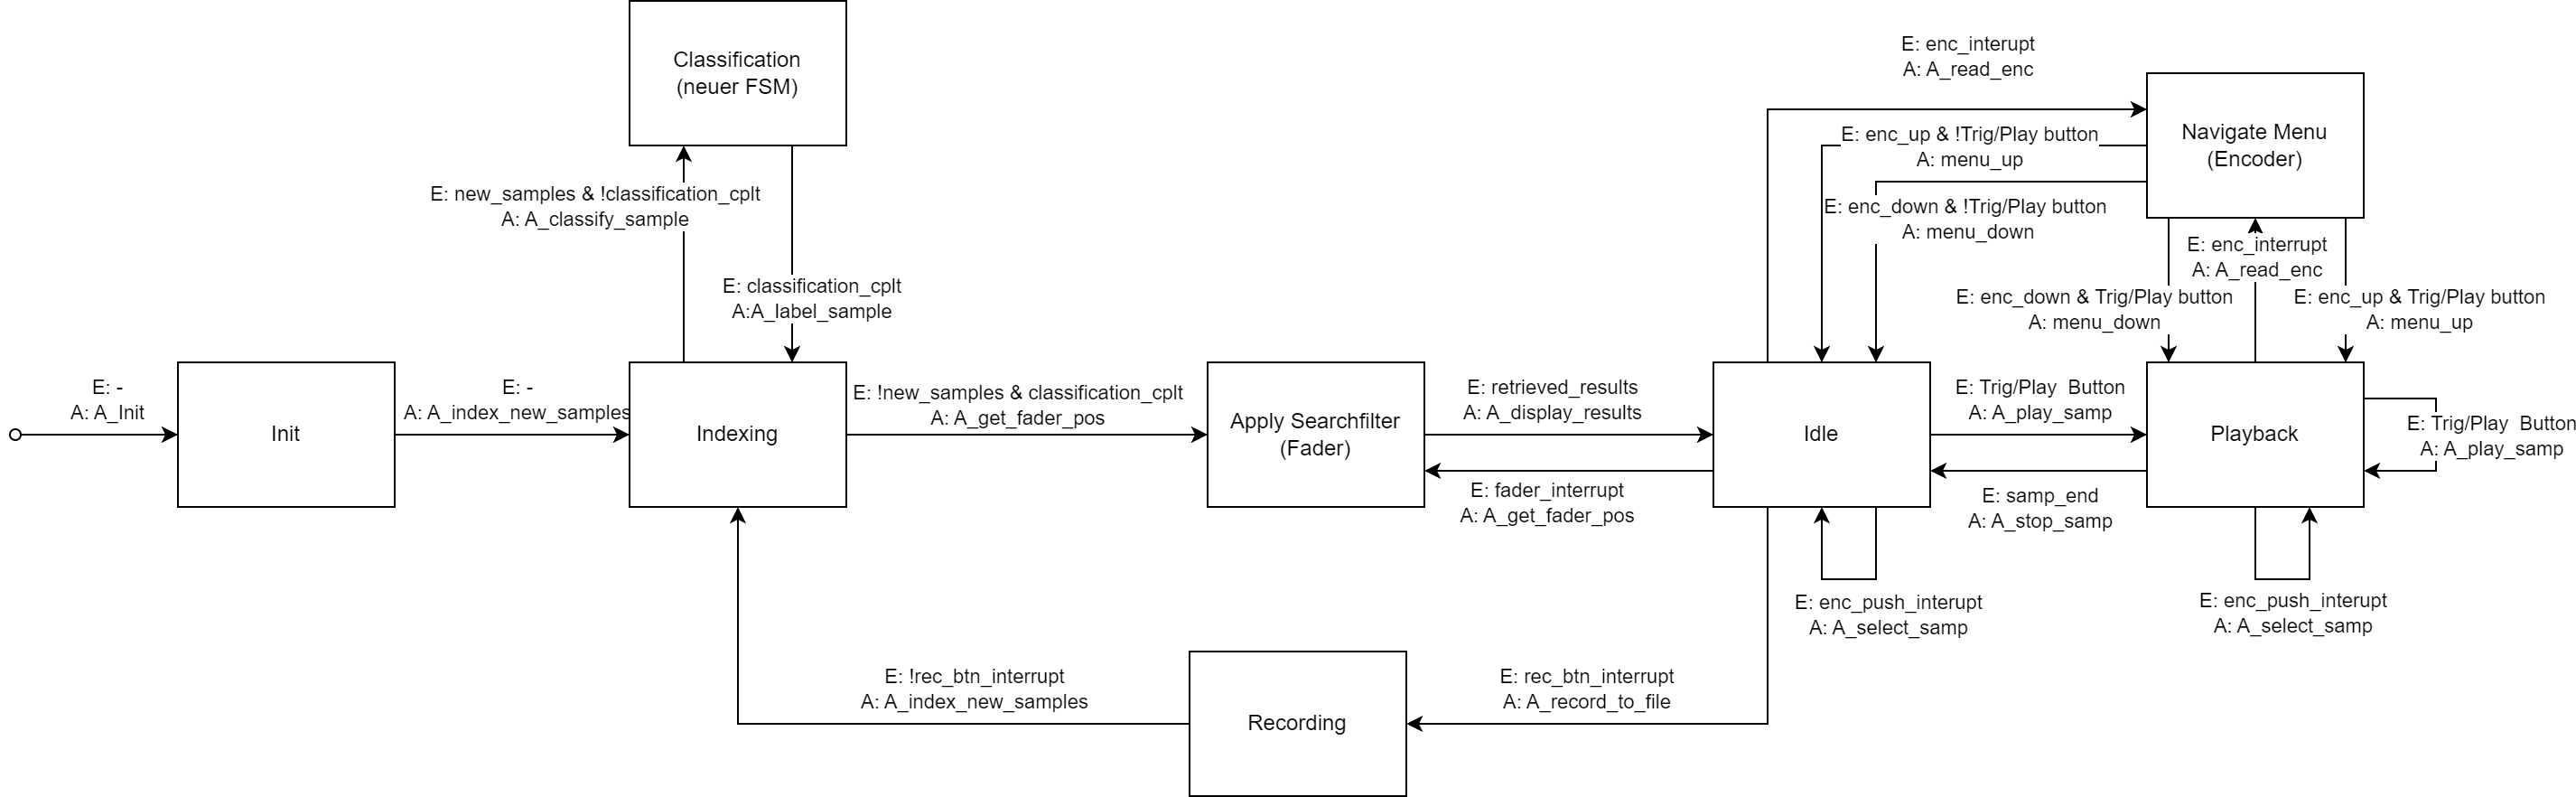
\includegraphics[width=1.0\textwidth]{images/04_spezifikation/fsm.drawio.png}
    	\caption{Zustandsautomat des Systems}
    	\label{fig:fsm}
    \end{figure}
    

\end{itemize}